\documentclass[10pt]{article}

\usepackage{neuripsstyle}
\usepackage[utf8]{inputenc}
\usepackage[T1]{fontenc}
\usepackage{amsmath,amssymb,bm}
\usepackage{booktabs}
\usepackage{array,multirow}
\usepackage{longtable}
\usepackage{graphicx}
\usepackage{adjustbox}
\usepackage{siunitx}
\usepackage{float}
\usepackage{placeins}
\usepackage{pdflscape}
\usepackage{caption}
\usepackage[hidelinks]{hyperref}
\captionsetup{font=small,labelfont=bf}
\renewcommand{\arraystretch}{1.12}
\graphicspath{{figs/}}

% --- notation ---
\newcommand{\zeq}{z^{\mathrm{eq}}_t}
\newcommand{\zbd}{z^{\mathrm{bd}}_t}
\newcommand{\Reg}{\mathcal{S}}
\newcommand{\Path}{\mathcal{P}}
\newcommand{\Acoup}{\textsc{coupled}}
\newcommand{\Bindep}{\textsc{independent}}
\sisetup{detect-weight=true,detect-family=true}

\title{Regime-Aware Tactical Asset Allocation for Equities and Fixed Income:\\
Independent and Coupled Jump-Model Labels}

\author{%
Team RLMM\\
\normalsize Machine Learning for Finance and Complex Systems}
\date{\today}

\begin{document}
\maketitle
\thispagestyle{empty}


\begin{abstract}
\noindent We study monthly tactical allocation across equities, bonds, and cash when the stock--bond diversification relation changes over time. The empirical design has three stages. First, jump-model teachers label realised equity and bond environments from return-based features. Second, supervised students forecast the next-month teacher labels from lagged macro-financial predictors. Third, the forecast probabilities are mapped into regime-conditional mean--variance allocations with transaction costs and turnover penalties.

\noindent We compare two label structures. The \Bindep{} approach estimates separate two-state labels for equities and bonds. The \Acoup{} approach estimates a three-state joint stock--bond label with calm, normal, and stressed regimes. Both approaches separate favourable and adverse return environments and identify the main economic distinction for balanced portfolios: bonds support equity drawdowns in episodes such as the dot-com bust and the global financial crisis, while inflation-driven sell-offs such as 1994 and 2022 weaken the bond hedge. In the student stage, regularized logistic regression and random forests produce informative next-month regime probabilities. In the allocation stage, the dynamic strategies improve the 60/40 benchmark along different margins: lower drawdowns, higher Sharpe ratios, or higher terminal wealth, depending on risk aversion and turnover control.
\end{abstract}

\section{Introduction}
Balanced portfolios depend on the diversification relation between equities and bonds. This relation changes across macro-financial environments. In disinflationary equity sell-offs, bond returns often rise and reduce portfolio losses. In inflation-driven sell-offs, equities and bonds can both lose value. A tactical allocation rule therefore needs information about the current stock--bond environment before it changes equity, bond, and cash weights.

This paper studies monthly regime-aware allocation for a broad equity leg and a broad fixed-income leg. The empirical objects are asset-class return environments. The equity leg represents the stock component of a balanced portfolio, and the bond leg represents the fixed-income component. The allocation problem is to decide whether the information available at the end of month \(t\) supports a change in next-month exposure after transaction costs and turnover penalties.

The empirical design has three stages. The teacher stage forms realised regime labels from equity and bond returns. The student stage forecasts the next-month teacher label from lagged macro-financial predictors. The allocation stage converts forecast probabilities into regime-conditional return moments and monthly portfolio weights. The regime label summarizes a persistent return environment. The allocation test then evaluates the economic value of the forecast probabilities.

We compare two regime-label structures. The \Bindep{} approach estimates separate binary labels for the equity and bond legs. Each leg is classified as favourable or unfavourable. The \Acoup{} approach estimates a joint stock--bond label with calm, normal, and stressed states. The independent structure keeps the two asset-level signals separate. The coupled structure gives a direct label for the joint diversification environment.

The empirical analysis is organised as follows. Section~\ref{sec:data} describes the return series, teacher features, and student predictors. Section~\ref{sec:teacher} defines the jump-model teachers and reports the label diagnostics. Section~\ref{sec:student} reports next-month prediction results. Section~\ref{sec:alloc} evaluates the regime-aware allocation rules against the 60/40 benchmark. The appendices report formulas, estimation details, diagnostic figures, and parameter-sensitivity checks.

\section{Data}
\label{sec:data}
The empirical analysis uses monthly excess returns for a broad equity leg and a broad bond leg. The equity leg is based on the S\&P~500 total return. The bond leg is based on an aggregate bond-index return. A one-month risk-free rate defines excess returns,
\[
r^{\mathrm{eq}}_t=\text{equity return}_t-rf_t,\qquad
r^{\mathrm{bd}}_t=\text{bond return}_t-rf_t .
\]
The bond leg contains both duration exposure and spread-sensitive components, so the student predictor panel includes Treasury-market variables and corporate-credit variables.

The teacher and student stages use different information sets. The teacher stage uses realised return information from the equity and bond legs to form regime labels. The student stage uses lagged macro-financial predictors to forecast those labels out of sample. This separation defines realised labels before the supervised forecasting problem is estimated.

\paragraph{Teacher features.}
The teacher features describe recent return performance, downside risk, volatility, and risk-adjusted performance. In the \Bindep{} specification, the equity teacher is estimated from daily equity excess returns using exponentially weighted returns and Sortino ratios over 21, 63, 126, and 252 trading days. The bond teacher is estimated from monthly bond excess returns using exponentially weighted returns, downside-risk measures, rolling Sharpe ratios, and volatility over horizons from one to twelve months. Table~\ref{tab:teacher-features} summarizes the teacher feature blocks. Appendix~\ref{app:features} reports the formulas.

\begin{table}[H]
\centering
\caption{Teacher features by approach. The \Bindep{} teacher uses daily equity features and monthly bond features. The \Acoup{} teacher uses a monthly joint stock--bond construction. Horizons are reported in trading days for daily equity features and in months for monthly features.}
\label{tab:teacher-features}
\small
\begin{adjustbox}{center,max width=1.08\textwidth}
\begin{tabular}{p{2.1cm}p{2.3cm}p{6.4cm}p{3.0cm}}
\toprule
Approach & Feature & Definition & Horizons \\
\midrule
\Bindep{} (equity) & Exponentially weighted return; Sortino ratio & Daily equity excess-return features based on recent mean performance and downside-risk-adjusted performance & 21, 63, 126, 252 trading days \\
\Bindep{} (bond) & Exponentially weighted return; downside risk; Sharpe ratio; volatility & Monthly bond excess-return features based on recent mean performance, negative-return magnitude, rolling risk-adjusted performance, and volatility & 1, 3, 6, 12 months \\
\midrule
\Acoup{} (eq, bd) & Sortino ratio & Recent average excess return over downside risk (EWMA of squared negative excess returns) & 1, 2, 4, 12 m \\
\Acoup{} (eq, bd) & Drawdown level / term structure & Log downside deviation; short minus long log downside deviation & 6 m; 2 vs 12 m \\
\Acoup{} (eq, bd) & MA crossover / trend & Short minus long average excess return, scaled by downside risk; EWMA-standardised trend & 3 vs 12 m; 12, 24 m \\
\bottomrule
\end{tabular}
\end{adjustbox}
\end{table}

\paragraph{Student panel.}
The \Bindep{} student panel is monthly and lagged. It combines equity factor returns, industry and size--value portfolio returns, Treasury returns, credit-fund returns, commodity returns, financial-condition indexes, interest-rate variables, inflation, volatility, macro activity, sentiment, and stock--bond correlation measures. The base panel contains 134 predictors. Each predictor is winsorised with past information, transformed into a causal rolling z-score, and smoothed with an exponentially weighted average. The student models use these lagged predictors to forecast the next-month teacher label.

The \Acoup{} student uses a separate monthly predictor construction with causal screening and current-regime context. Its predictors are described with the coupled results.

\section{Teacher: regime labelling with statistical jump models}
\label{sec:teacher}

The teacher stage converts realised equity and bond returns into regime labels. These labels
define the supervised targets used by the student models. A regime label must be
persistent enough to describe a market environment and separated enough to have an economic
interpretation. The teacher diagnostics therefore report persistence, state-conditional
returns, crisis-window behaviour, and feature separation before the labels enter the
prediction and allocation stages.

\subsection{The jump model}

A jump model assigns each observation to one of a finite number of states and penalises state
changes. For a standardised feature vector \(x_t\) and state \(s_t\), the fitted path
minimises
\begin{equation}
\min_{s_1,\dots,s_T,\,\{c_k\}}\ \sum_{t=1}^{T} d(x_t,c_{s_t})\;+\;\lambda\sum_{t=2}^{T}\Lambda(s_{t-1},s_t),
\label{eq:jump-generic}
\end{equation}
where \(d(\cdot,c_k)\) is the distance to state centre \(c_k\), \(\Lambda\) is the switching
penalty, and \(\lambda\) controls persistence. Larger \(\lambda\) values produce longer
spells. Conditional on centres, the state path is decoded by dynamic programming.
Conditional on the state path, the centres are re-estimated. The two steps are iterated from
several initialisations.

\subsection{Two regime parameterisations}
\label{sec:two-parameterisations}

Both approaches use a jump penalty, with different state spaces.

\paragraph{\Bindep{}: two independent binary labels.}
The \Bindep{} teacher estimates separate two-state jump models for the equity and bond legs.
For asset \(a\in\{\mathrm{eq},\mathrm{bd}\}\), feature vector \(x^a_i\), and teacher member
\(p\), the fitted path solves
\begin{equation}
\min_{s^a_1,\dots,s^a_{T_a},\,\{c^a_0,c^a_1\}}
\sum_{i=1}^{T_a} d_p\!\left(x^a_i,c^a_{s^a_i}\right)
+\lambda_p\sum_{i=2}^{T_a}\mathbf{1}\{s^a_i\neq s^a_{i-1}\}.
\label{eq:independent-teacher}
\end{equation}
For equities, the index \(i\) is daily. For bonds, the index \(i\) is monthly. The equity
teacher is first estimated after a 12-year daily training window and is then refit at month
ends. The bond teacher is first estimated after a 144-month training window and is then refit
monthly. At each refit date, the available training features are standardised before fitting.

The path set \(p\in\Path_a\) combines two distance choices and a grid of jump penalties. The
standard distance uses squared Euclidean loss and mean centres. The robust distance uses
\(L^1\) loss and medoid centres. The equity grid uses
\(\lambda_p\in\{2,4,8,16,32,64,128\}\). The bond grid uses fifteen values from \(0\) to
\(4\), with finer spacing near zero.

States are ordered after each fit by realised in-sample Sharpe ratio. Let \(g^{a,p}\) denote
the higher-Sharpe state. This state is labelled favourable. The monthly label
from path \(p\) is
\begin{equation}
S^{\mathrm{eq},p}_m
=
\mathbf{1}\!\left\{
\frac{1}{n_m}\sum_{i\in m}\mathbf{1}\{s^{\mathrm{eq},p}_i=g^{\mathrm{eq},p}\}
\ge \frac{1}{2}
\right\},
\qquad
S^{\mathrm{bd},p}_m
=
\mathbf{1}\{s^{\mathrm{bd},p}_m=g^{\mathrm{bd},p}\}.
\label{eq:independent-monthly-label}
\end{equation}
The equity label is therefore the majority daily state within the month. The bond label is
the fitted monthly state.

\paragraph{\Acoup{}: three joint regimes with a coupling probability.}
The \Acoup{} approach represents the stock--bond environment with three joint regimes. Each
leg has a benign or adverse bit, and the admissible joint states are
\[
\Reg=\{\,\text{calm}=(0,0),\ \ \text{normal}=(1,0),\ \ \text{stressed}=(1,1)\,\},
\]
where the pair is the equity bit and the bond bit. Calm means that both legs are benign,
normal means that equity is adverse while bonds remain benign, and stressed means that both
legs are adverse. The benign-equity/adverse-bond state is excluded in this specification.

For a joint state $j$ with bits $(j_E,j_B)$, the per-month cost combines the two leg-specific
distances with a coupling term:
\begin{equation}
e_t(j)=d\!\left(\zeq,\mu^{\mathrm{eq}}_{j_E}\right)+d\!\left(\zbd,\mu^{\mathrm{bd}}_{j_B}\right)
+\eta\Big[\,\kappa_t\,\mathbf{1}\{j\in D\}+(1\kappa_t)\,\mathbf{1}\{j\in A\}\,\Big],
\label{eq:emission}
\end{equation}
where $A$ denotes the agree states, calm and stressed, and $D$ denotes the disagree state,
normal. The scalar $\eta$ controls the strength of the coupling term. The variable
$\kappa_t\in[0,1]$ is a learned coupling probability: low values favour the disagree state, while
high values favour the agree states. Given the current state path, $\kappa_t$ is fitted by an
$L^2$-penalised logistic regression of the leg-agreement indicator
$y_t=\mathbf{1}\{s^{\mathrm{eq}}_t=s^{\mathrm{bd}}_t\}$ on equity--bond correlation, equity
and bond trend, and equity and bond drawdown:
\begin{equation}
\kappa_t=\sigma\!\left(\beta_0+\beta^{\top}x^{\mathrm{mkt}}_t\right),\qquad
x^{\mathrm{mkt}}_t=\big\{\rho^{\,\mathrm{eq,bd}}_{12,t},\ \mathrm{trend}^{\mathrm{eq}}_t,\
\mathrm{trend}^{\mathrm{bd}}_t,\ \mathrm{dd}^{\mathrm{eq}}_t,\ \mathrm{dd}^{\mathrm{bd}}_t\big\}.
\label{eq:wt}
\end{equation}
The transition penalty is applied separately to the equity and bond bits,
$\Lambda(i,j)=\lambda\,\mathbf{1}\{i_E\neq j_E\}+\lambda\,\mathbf{1}\{i_B\neq j_B\}$.
The coupling term acts as a soft bias in the state cost. It raises the cost of states that
conflict with the fitted stock--bond dependence signal and lowers the cost of states
supported by that signal.

\paragraph{Relationship.}
The two parameterisations define different regime objects. The \Bindep{} labels keep the
equity and bond states separate and allow all four favourable--unfavourable combinations. The
\Acoup{} labels impose a three-state joint structure: calm corresponds to favourable equity
and favourable bonds, normal corresponds to unfavourable equity and favourable bonds, and
stressed corresponds to unfavourable equity and unfavourable bonds. The independent
representation supplies separate asset-level signals. The coupled representation supplies a
direct label for the joint stock--bond environment.

\subsection{Ensembling and voting}

The \Bindep{} teacher aggregates the fitted paths separately for each asset. For asset \(a\),
the vote probability is
\begin{equation}
\pi^a_m=\frac{1}{|\Path_a|}\sum_{p\in\Path_a}S^{a,p}_m,
\qquad
S^a_m=\mathbf{1}\{\pi^a_m\ge 1/2\}.
\label{eq:independent-vote}
\end{equation}
The final independent teacher label is the majority-vote state \(S^a_m\), and \(\pi^a_m\)
measures agreement across fitted paths. This gives one favourable-state probability for
equities and one favourable-state probability for bonds.

The \Acoup{} teacher fits 22 coupled members, formed from eleven feature families crossed
with the \(L^1\) and \(L^2\) norms, and aggregates the members by equal-weight majority vote.
It reports the regime vote shares and the average coupling probability across members. In
both approaches, the vote share measures agreement across fitted paths.

\subsection{Label results}
\label{sec:teacher-results}

Both teacher specifications produce persistent regimes with clear return differences across
states. These diagnostics establish that the labels are suitable supervised targets for the
student stage.

Figure~\ref{fig:labels} compares the two label representations. The \Bindep{} panel shows
equity and bond excess-return indexes with favourable-regime months marked for each leg. The
\Acoup{} panel shows the same stock--bond history using the three joint regimes.
Figure~\ref{fig:vote-wt} reports the coupled ensemble vote shares and the estimated coupling
probability.

\begin{figure}[H]
\centering
\begin{minipage}{0.46\textwidth}
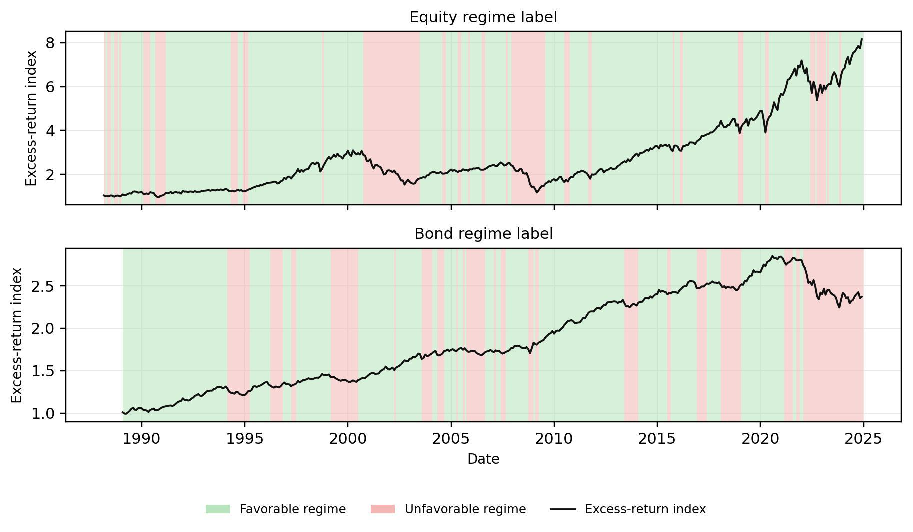
\includegraphics[width=\linewidth]{teacher_regime_labels.pdf}
\end{minipage}\hfill
\begin{minipage}{0.52\textwidth}

\includegraphics[width=\linewidth]{COUPLED__labels.png}
\end{minipage}
\caption{Regime-label representations of the stock--bond history. Left (\Bindep): equity and
bond excess-return indexes with favourable-regime months marked for each leg. Right
(\Acoup): cumulative excess-return indexes shaded by calm, normal, and stressed joint
regimes; inset numbers report within-span annualised Sharpe ratios.}
\label{fig:labels}
\end{figure}

\begin{figure}[H]
\centering

\includegraphics[width=\linewidth]{COUPLED__vote_kappa.png}
\caption{\Acoup{} ensemble label construction. The top panel reports per-class vote shares
across the 22 coupled members. The bottom panel reports the average coupling probability
$kappa_t$ with the regime shading and the $0.5$ reference line.}
\label{fig:vote-wt}
\end{figure}

\paragraph{State economics.}
Table~\ref{tab:state-economics} reports label-conditional excess-return statistics. In the
\Bindep{} panel, favourable equity months have a Sharpe ratio of $1.14$, compared with
$-0.75$ in unfavourable months. Favourable bond months have a Sharpe ratio of $1.81$,
compared with $-0.81$ in unfavourable months.
In the \Acoup{} panel, equity earns a Sharpe
ratio of $+2.60$ in calm, $+0.67$ in normal, and $-2.99$ in stressed, while bonds earn $+0.22$,
$+1.00$, and $-1.69$ across the same three regimes. Equity performance is therefore highest in
calm, weaker in normal, and negative in stressed, and bond performance is positive in calm and
normal and negative in stressed. This ordering is consistent with the
interpretation of normal as a diversifying equity-drawdown state and stressed as a state in
which both legs are adverse.


\begin{table}[H]
\caption{Label-conditional economics. Statistics use the same-month annualised excess return
of the labelled leg. The \Bindep{} panel conditions on each leg's binary label; the \Acoup{}
panel conditions on the three joint regimes. Share is the fraction of labelled months;
duration is the average spell length (months).}
\label{tab:state-economics}
\small
\begin{adjustbox}{left,max width=1.08\textwidth}
\begin{tabular}{@{}llrrrrr@{}}
\toprule
\multicolumn{7}{l}{\textbf{\Bindep{}: two binary labels (through Nov 2024)}}\\
\midrule
Class & Regime & Share & Ann.\ ret. & Ann.\ vol. & Sharpe & Avg.\ dur. \\
\midrule
Equity & Favourable   & 75.6\% & $+13.7\%$ & $12.0\%$ & $+1.14$ & 12.8 \\
Equity & Unfavourable & 24.4\% & $-14.5\%$ & $19.4\%$ & $-0.75$ & \phantom{0}4.2 \\
Bond   & Favourable   & 67.1\% & $+5.7\%$  & $3.2\%$  & $+1.81$ & 13.8 \\
Bond   & Unfavourable & 32.9\% & $-4.1\%$  & $5.0\%$  & $-0.81$ & \phantom{0}6.8 \\
\midrule
\multicolumn{7}{l}{\textbf{\Acoup{}: three joint regimes (1988-02--Nov 2024)}}\\
\midrule
Class & Regime & Share & Ann.\ ret. & Ann.\ vol. & Sharpe & Avg.\ dur. \\
\midrule
Equity & Calm     & 13.8\% & $+21.0\%$ & $8.1\%$  & $+2.60$ & \phantom{0}4.7 \\
Equity & Normal   & 77.1\% & $+9.9\%$  & $14.8\%$ & $+0.67$ & 12.2 \\
Equity & Stressed & \phantom{0}9.0\% & $-40.9\%$ & $13.7\%$ & $-2.99$ & \phantom{0}2.2 \\
Bond   & Calm     & 13.8\% & $+0.8\%$  & $3.5\%$  & $+0.22$ & \phantom{0}4.7 \\
Bond   & Normal   & 77.1\% & $+3.9\%$  & $3.9\%$  & $+1.00$ & 12.2 \\
Bond   & Stressed & \phantom{0}9.0\% & $-8.4\%$  & $5.0\%$  & $-1.69$ & \phantom{0}2.2 \\
\bottomrule
\end{tabular}
\end{adjustbox}
\end{table}






\paragraph{Persistence.}
The regimes are persistent in both specifications. Through November 2024, the \Bindep{}
labels switch 51 times for equities and 41 times for bonds. The favourable states have
average durations of \(12.8\) months for equities and \(13.8\) months for bonds. In the
\Acoup{} sample, the coupled ensemble records 58 regime switches across 442 months. Normal
is the most persistent joint regime, with an average duration of \(12.2\) months. Stressed is
shorter-lived, with an average duration of \(2.2\) months. The transition matrices are
reported in Appendices~\ref{app:teacher-independent} and \ref{app:teacher-coupled}.

\paragraph{Crisis windows.}
Table~\ref{tab:crisis} compares the labels across historical stress windows. During the
dot-com bust and the global financial crisis, the bond leg remains mostly favourable in the
\Bindep{} specification and the \Acoup{} specification assigns most months to normal. In
these episodes, bonds retain positive Sharpe ratios and diversify weak equity returns. In the
1994 bond shock and the 2022 inflation sell-off, the bond label is mostly unfavourable in the
\Bindep{} specification and the \Acoup{} specification assigns a large share of months to
stressed. These windows identify the central stock--bond distinction for allocation: normal
describes equity weakness with bond support, while stressed describes a joint adverse
environment.

\begin{table}[H]
\centering
\caption{Crisis-window behaviour under both labellings. The \Bindep{} columns report the bond
label's favourable share and Sharpe; the \Acoup{} columns report the joint regime mix within
each window and the equity/bond Sharpe. Sharpe ratios use same-month annualised excess
returns over each window.}
\label{tab:crisis}
\small
\begin{adjustbox}{center,max width=1.08\textwidth}
\begin{tabular}{lrrrrrrr}
\toprule
& \multicolumn{2}{c}{\Bindep{} bond} & \multicolumn{3}{c}{\Acoup{} regime share} & \multicolumn{2}{c}{\Acoup{} Sharpe} \\
\cmidrule(lr){2-3}\cmidrule(lr){4-6}\cmidrule(lr){7-8}
Window & Fav. & Sharpe & Calm & Normal & Stress. & Eq. & Bd. \\
\midrule
1990 recession          & 100.0\% & $+1.33$ & 0\%  & 100\% & \phantom{0}0\%  & $+0.05$ & $+1.41$ \\
1994 bond shock         & \phantom{0}8.3\% & $-1.55$ & 8\%  & 33\%  & 58\% & $-0.48$ & $-1.61$ \\
Dot-com bust            & 87.5\% & $+1.81$ & 0\%  & 97\%  & \phantom{0}3\%  & $-1.07$ & $+1.97$ \\
Global financial crisis & 72.2\% & $+0.74$ & 0\%  & 94\%  & \phantom{0}6\%  & $-1.58$ & $+0.74$ \\
Euro sovereign 2011     & 100.0\% & $+3.46$ & 12\% & 88\%  & \phantom{0}0\%  & $-0.61$ & $+3.69$ \\
Covid crash             & 100.0\% & $+2.25$ & 0\%  & 100\% & \phantom{0}0\%  & $-0.88$ & $+2.76$ \\
Inflation 2022          & \phantom{0}0.0\% & $-1.82$ & 0\%  & 33\%  & 67\% & $-0.93$ & $-1.90$ \\
\bottomrule
\end{tabular}
\end{adjustbox}
\end{table}

\paragraph{Feature separation.}
The feature-separation diagnostics rank inputs by how strongly their fitted state centres
differ. In the \Bindep{} specification, the equity label is separated mainly by
medium-horizon Sortino ratios and exponentially weighted returns. The bond label is separated
mainly by 6- and 12-month Sharpe ratios and short-horizon downside-risk measures. In the
\Acoup{} specification, equity trend and risk-adjusted performance separate calm from the
other regimes, while bond trend and longer-horizon bond Sortino ratios distinguish stressed
from the other states. Full rankings are reported in Appendices~\ref{app:teacher-independent}
and \ref{app:teacher-coupled}.


\section{Student: forecasting the next-month regime}
\label{sec:student}

The student stage forecasts the next-month teacher label from information observed at the
end of the current month. For month \(t\), the target is the teacher label at \(t+1\). The
predictors are the lagged macro-financial variables described in Section~\ref{sec:data}. The
\Bindep{} student estimates separate binary forecasts for the equity and bond favourable
states. The \Acoup{} student estimates a three-class forecast for the joint calm, normal, and
stressed regimes.

For the independent student, let \(S^a_{t+1}\in\{0,1\}\) denote the next-month majority-vote
label for asset \(a\in\{\mathrm{eq},\mathrm{bd}\}\), and let \(X_t\) denote the predictor
vector observed at month \(t\). The fitted student produces
\begin{equation}
\hat p^a_{t+1|t}
=
\Pr\!\left(S^a_{t+1}=1\mid X_t\right),
\qquad a\in\{\mathrm{eq},\mathrm{bd}\}.
\label{eq:independent-student-probability}
\end{equation}
The probability \(\hat p^a_{t+1|t}\) is the input passed to the allocation stage.

The \Bindep{} student evaluates two predictor designs: smoothed z-scores only, and z-scores
together with smoothed z-scores. The models are \(L^2\)-penalised logistic regression and
random forests. Logistic regressions use class-balanced penalties. Random forests use shallow
trees and class-balanced subsampling. Hyperparameters are selected in a walk-forward
validation design. Each forecast uses at least 96 months for training and the next 36 months
for validation. The selected specification is refit on the combined training and validation
sample and then evaluated on the next out-of-sample month.

The \Acoup{} student uses multinomial logistic regression and random forests with causally
screened predictors and current-regime context. Both approaches report
out-of-sample prediction diagnostics before the forecasts enter the allocation stage.

\paragraph{Forecast quality.}
Table~\ref{tab:forecast} reports out-of-sample prediction diagnostics. In the \Bindep{}
panel, logistic regression gives the highest reported AUC for both labels. For the equity
label, logistic regression reaches an AUC of \(0.929\), compared with \(0.903\) for the
random forest. For the bond label, logistic regression reaches an AUC of \(0.892\), compared
with \(0.873\) for the random forest. Balanced accuracy, Brier score, and log loss give the
same ordering for the headline independent specifications. The full independent
predictor-design results are reported in Table~\ref{tab:student-oos-prediction-summary}.

The \Acoup{} panel reports the same four diagnostics for the joint three-class forecast. The
random forest and logistic regression attain similar AUC (0.776 and 0.770), so the two models
rank the regimes comparably. The random forest has the better Brier and log-loss scores, while
logistic regression attains the higher balanced accuracy. The allocation stage uses the
probability forecasts, so these diagnostics are interpreted together with the portfolio results
in Section~\ref{sec:alloc}.

\begin{table}[H]
\centering
\caption{Out-of-sample student forecast quality. The \Bindep{} panel reports binary
diagnostics for the equity and bond favourable-state forecasts. The full independent
predictor-design results are in Table~\ref{tab:student-oos-prediction-summary}. The
\Acoup{} panel reports the same four diagnostics for the joint three-class forecast, with
AUC as the macro one-vs-rest average and the Brier and log-loss scores in their multiclass
forms.}
\label{tab:forecast}
\small
\begin{adjustbox}{center,max width=1.08\textwidth}
\begin{tabular}{llcccc}
\toprule
\multicolumn{6}{l}{\textbf{\Bindep{}: per-leg binary forecast (OOS to 2024-12; equity starts 1995-03, bond starts 1996-02)}}\\
\midrule
Label & Model & AUC & Bal.\ acc. & Brier & Log loss \\
\midrule
Equity & Logistic regression & 0.929 & 0.846 & 0.088 & 0.296 \\
Equity & Random forest       & 0.903 & 0.831 & 0.107 & 0.361 \\
Bond   & Logistic regression & 0.892 & 0.831 & 0.128 & 0.462 \\
Bond   & Random forest       & 0.873 & 0.800 & 0.147 & 0.471 \\
\midrule
\multicolumn{6}{l}{\textbf{\Acoup{}: three-class forecast (OOS 1996-02 to 2024-10)}}\\
\midrule
\multicolumn{2}{l}{Model} & AUC & Bal.\ acc. & Brier & Log loss \\
\midrule
\multicolumn{2}{l}{Logistic regression} & 0.770 & 0.677 & 0.541 & 1.062 \\
\multicolumn{2}{l}{Random forest}       & 0.776 & 0.595 & 0.383 & 0.686 \\
\bottomrule
\end{tabular}
\end{adjustbox}
\end{table}

\begin{figure}[H]
\centering
\begin{minipage}{0.49\textwidth}
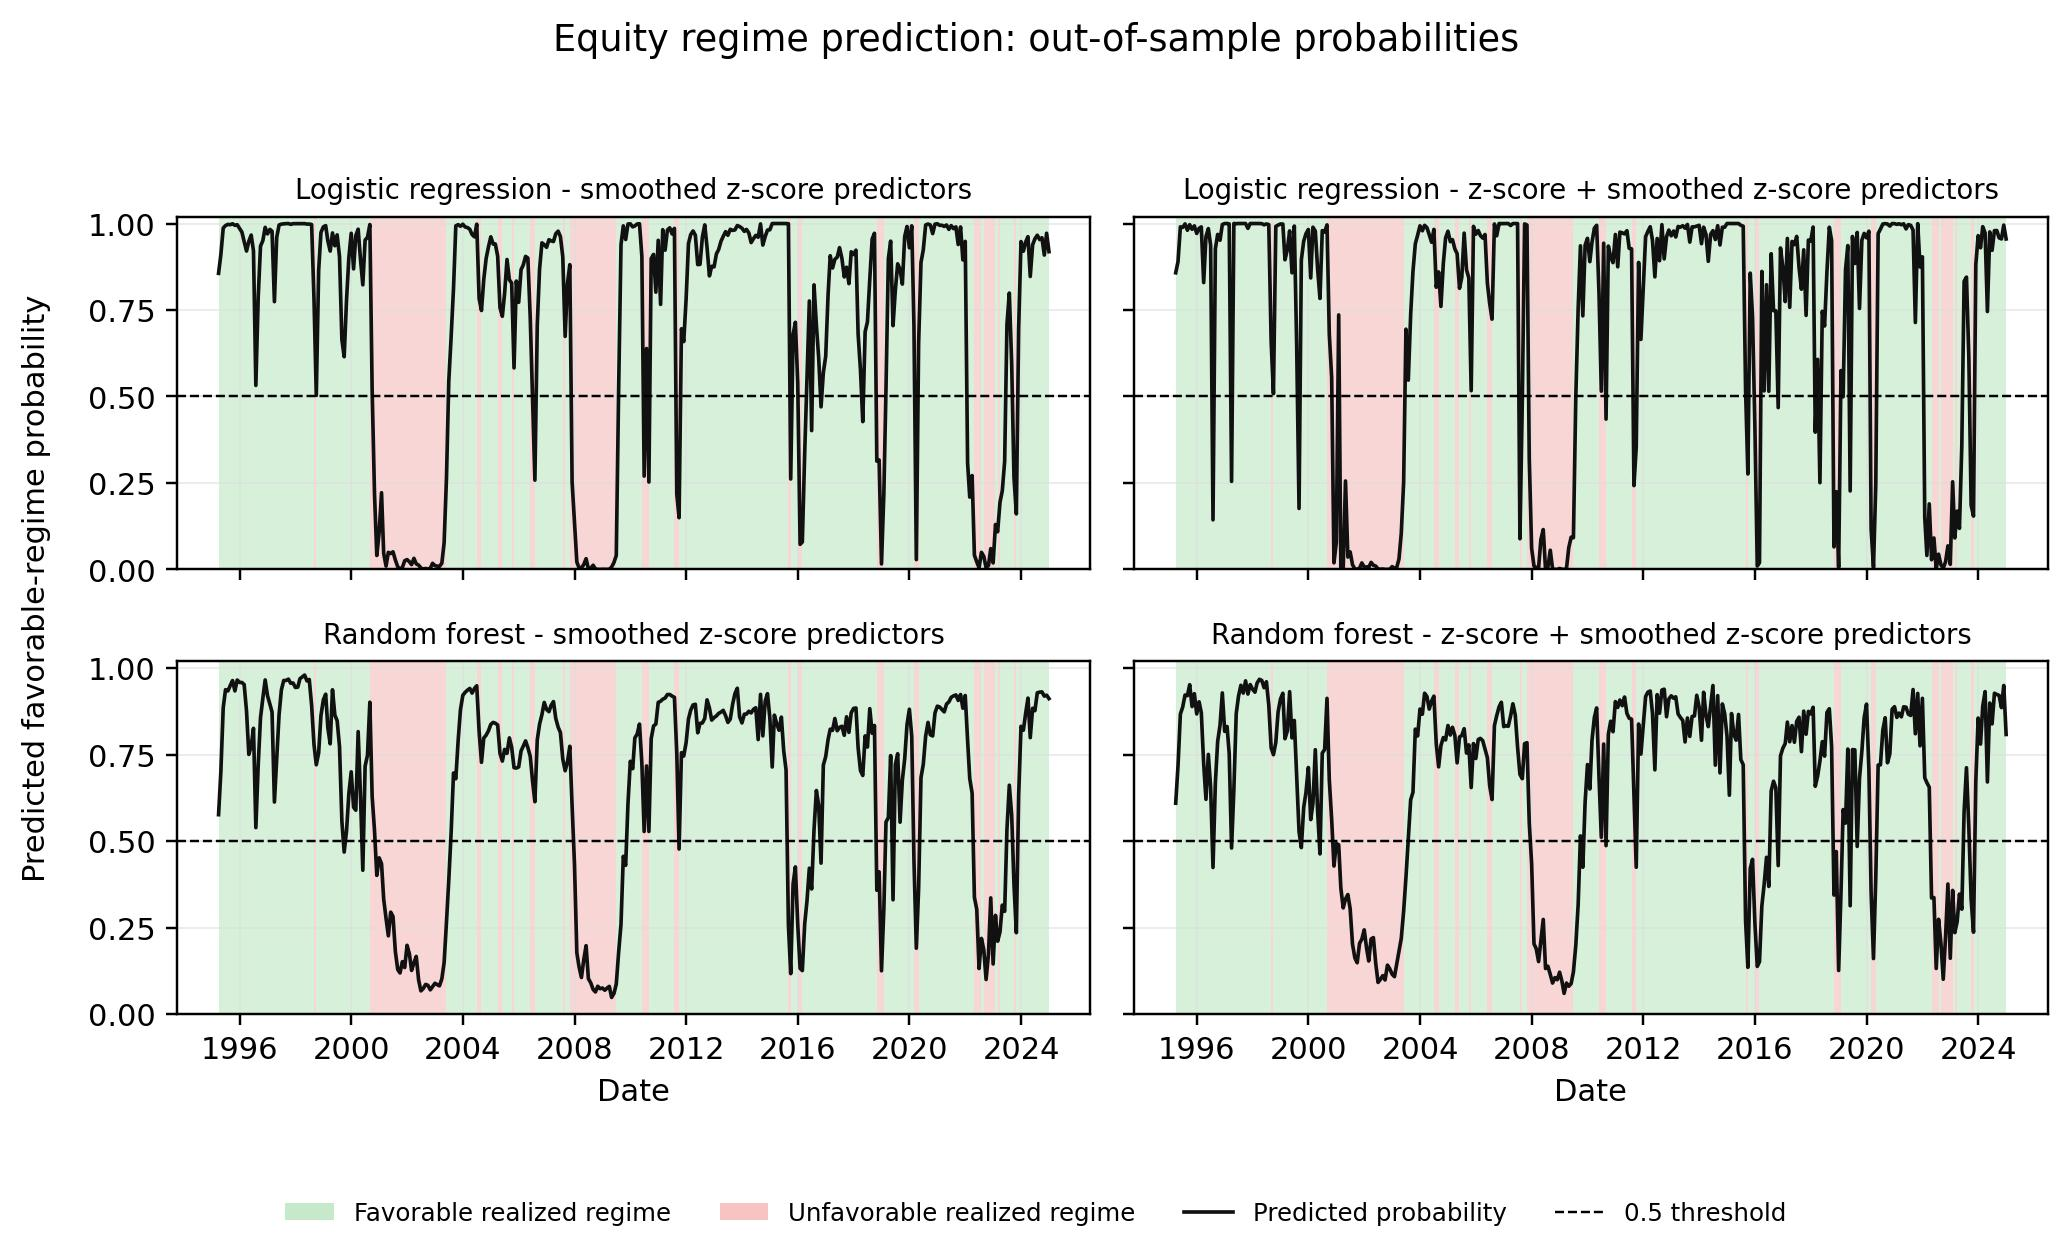
\includegraphics[width=\linewidth]{equity_prediction_probabilities.jpg}
\end{minipage}\hfill
\begin{minipage}{0.49\textwidth}
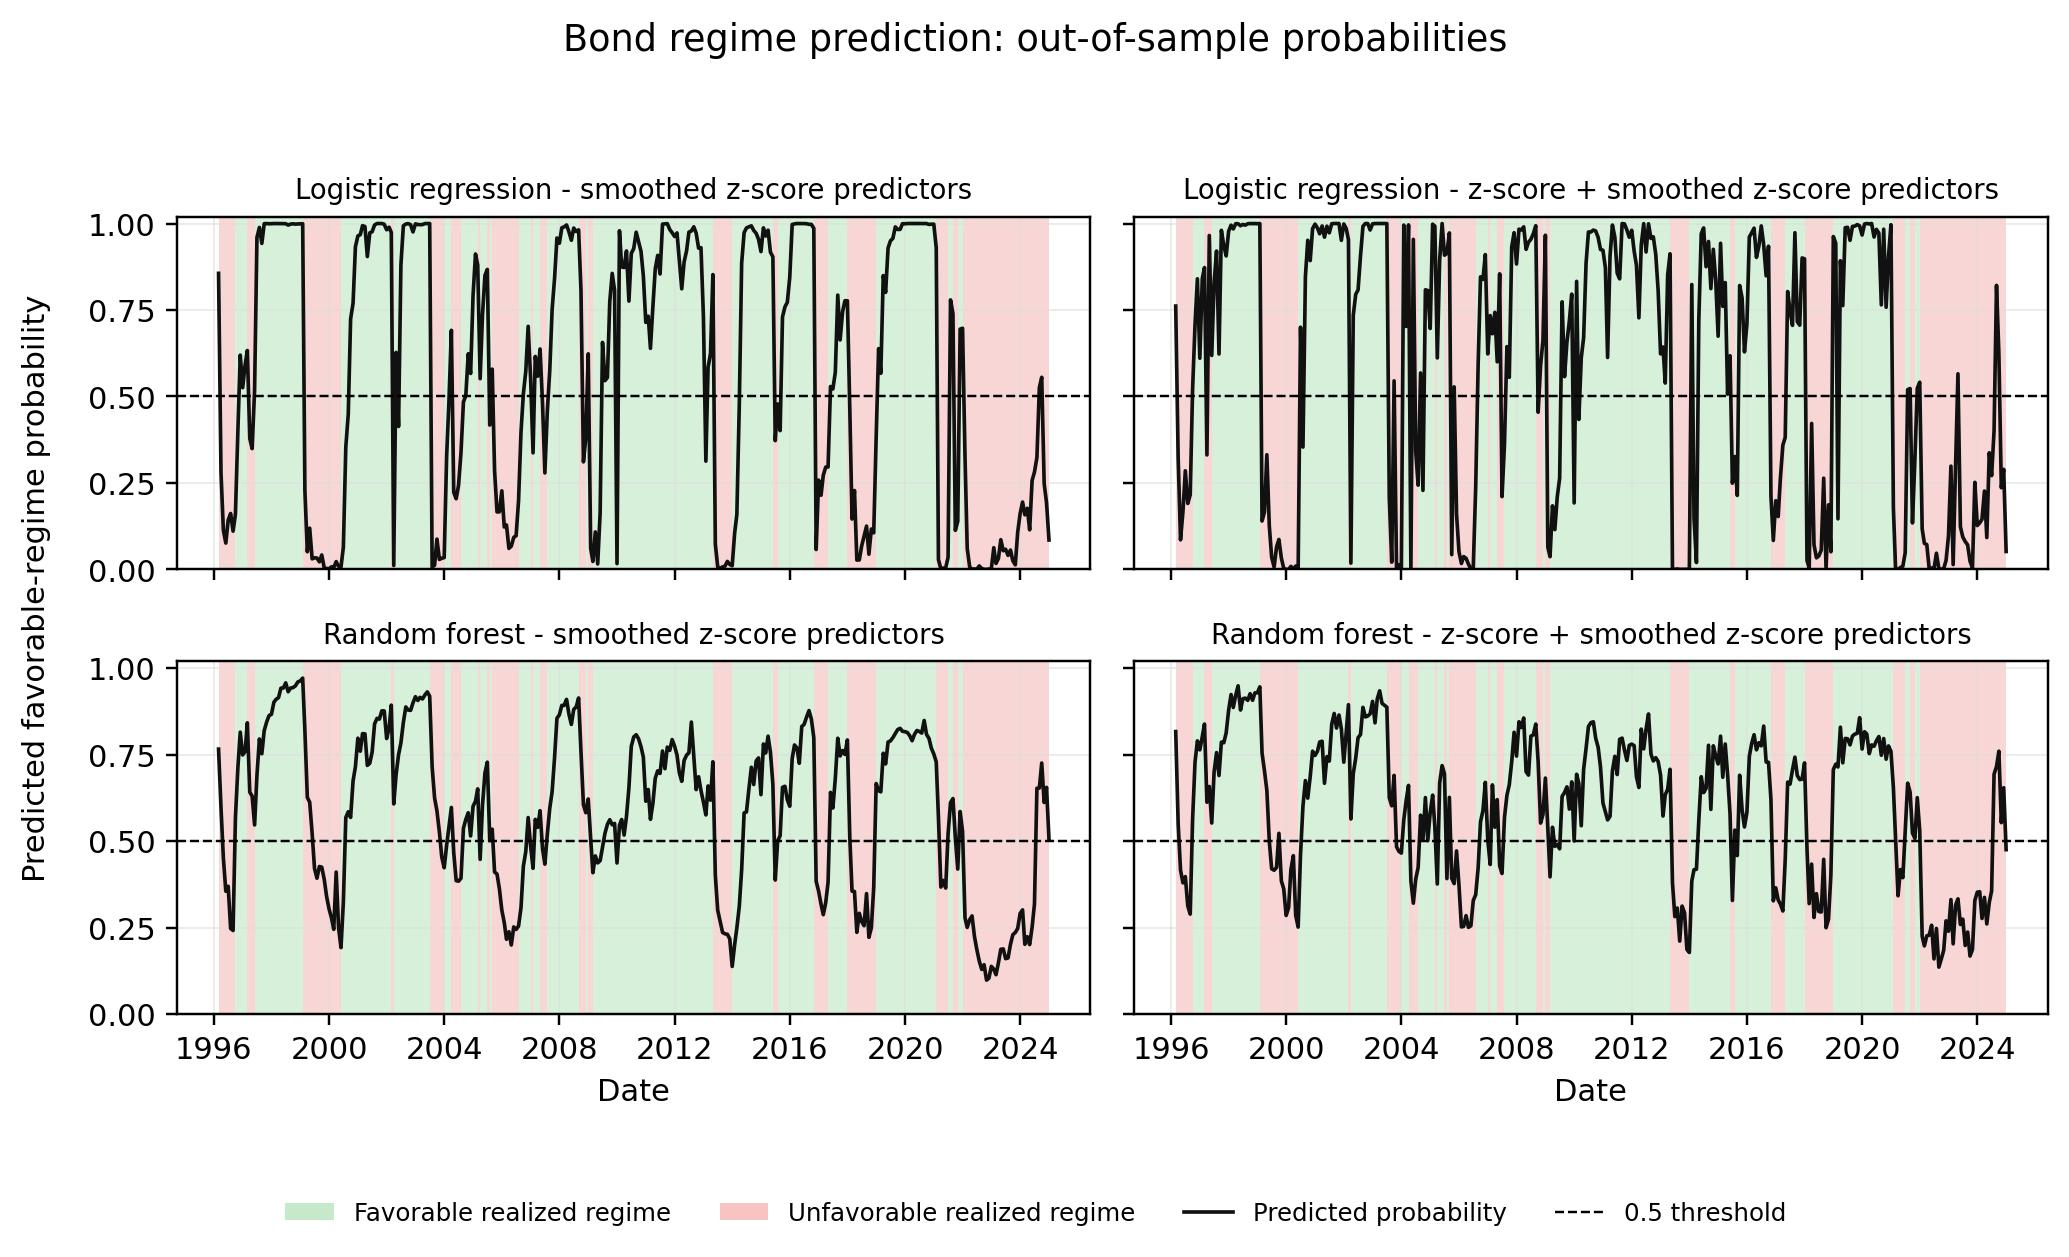
\includegraphics[width=\linewidth]{bond_prediction_probabilities.jpg}
\end{minipage}
\caption{\Bindep{} student out-of-sample probability paths. The left panel reports equity
favourable-regime probabilities, and the right panel reports bond favourable-regime
probabilities. Shading marks the realised teacher label, the black line reports the predicted
favourable-regime probability, and the dashed line marks the $0.5$ threshold.}
\label{fig:student-probs}
\label{fig:student-equity-probabilities}
\label{fig:student-bond-probabilities}
\end{figure}

\begin{figure}[H]
\centering

\includegraphics[width=\linewidth]{COUPLED__pred_probabilities.pdf}
\caption{\Acoup{} student out-of-sample probability paths for the three joint regimes
(calm, normal, stressed), shown for the logistic and random-forest students. Shading marks
the realised teacher regime, the black lines report the predicted regime probabilities, and
the dashed line marks the $0.5$ threshold.}

\label{fig:c-student-probs}
\end{figure}
Figure~\ref{fig:student-probs} reports the independent out-of-sample probability paths used
by the allocator. Equity favourable-state probabilities decline during the 2000--2003 and
2008--2009 equity drawdowns and increase during long favourable equity periods. Bond
favourable-state probabilities switch more often, consistent with the shorter bond-regime
spells in Table~\ref{tab:state-economics}. The allocator uses these probabilities as
continuous inputs when forming regime-conditional moments.

\paragraph{Predictor information.}
Figure~\ref{fig:importance} summarizes \Bindep{} feature importance by predictor block.
Logistic-regression importance is based on absolute coefficient magnitude. Random-forest
importance is impurity-based. The results differ by target. Equity-regime forecasts draw
mainly on equity cross-section and industry or style variables, with additional information
from Treasury, credit, commodity, and macro-financial predictors. Bond-regime forecasts use a
broader mix of equity cross-section, Treasury-market, and credit-market variables. This
pattern is consistent with separate asset-level labels: equity states depend strongly on
risk appetite and equity-market conditions, while bond states also depend on rates, credit
conditions, and the financing environment.

\begin{figure}[H]
\centering
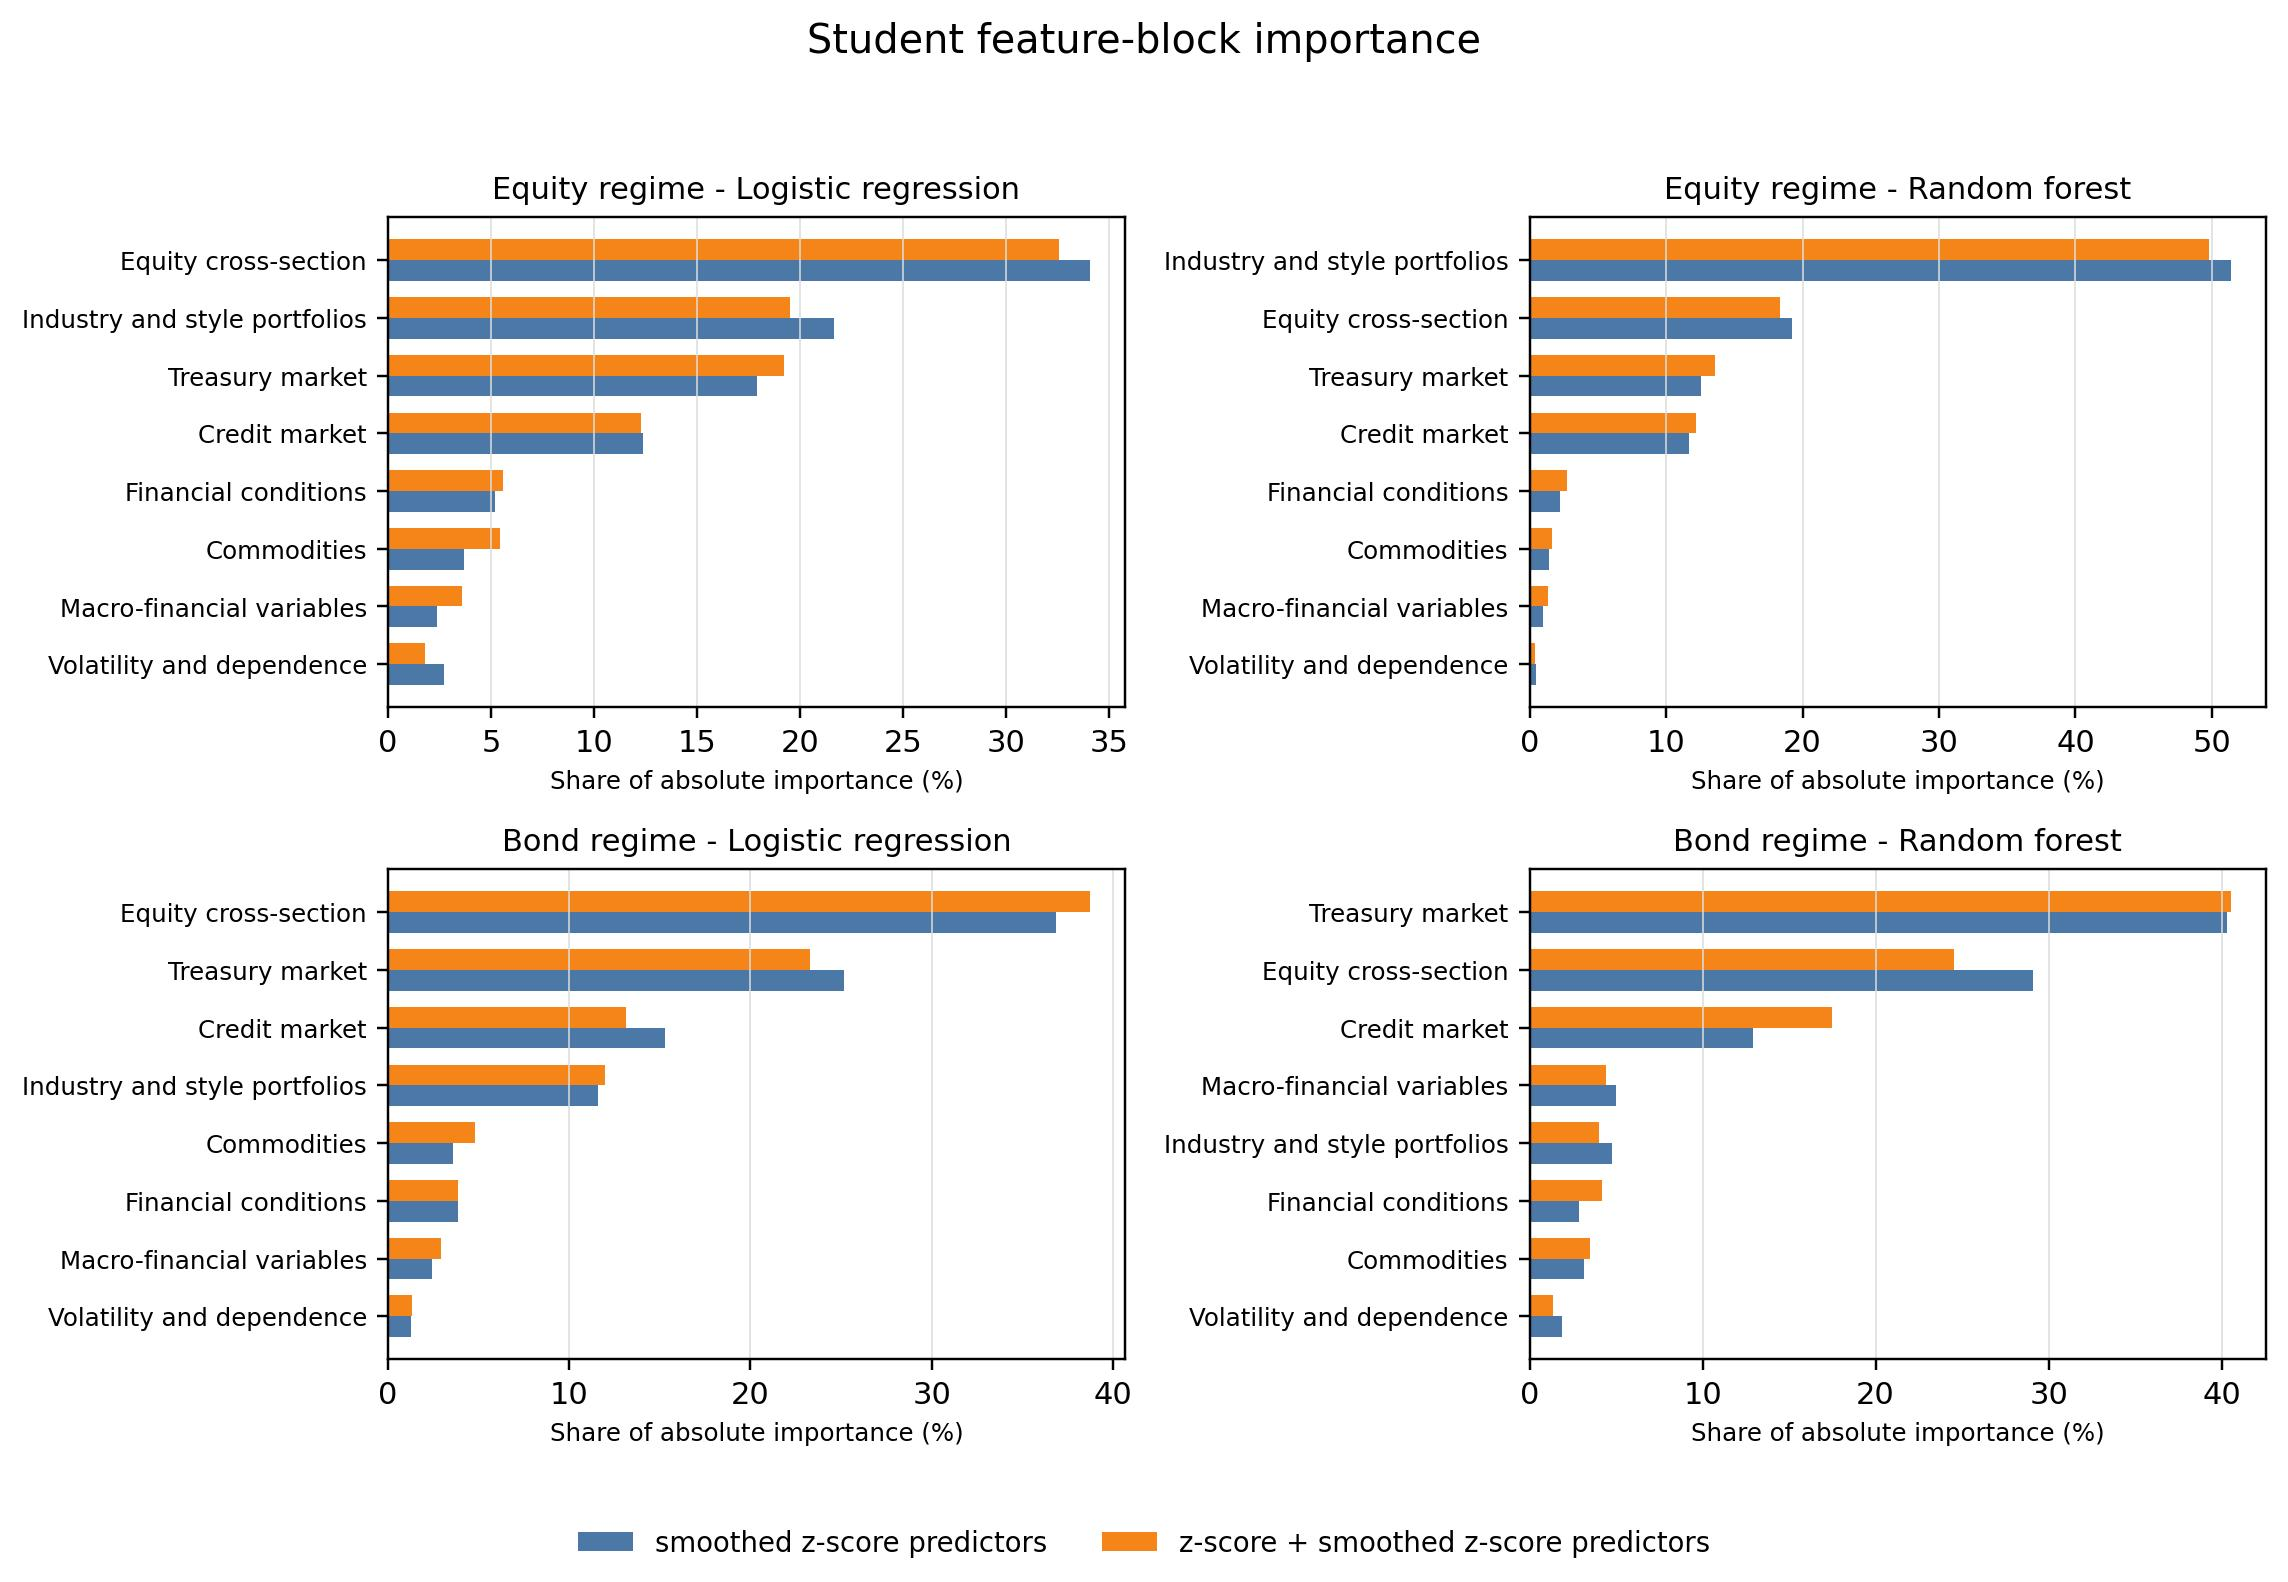
\includegraphics[width=\linewidth]{feature_block_importance.jpg}
\caption{\Bindep{} student feature-block importance. Logistic-regression importance is based
on absolute coefficient magnitude. Random-forest importance is impurity-based. Values are
aggregated within predictor blocks.}
\label{fig:importance}
\end{figure}

For the \Acoup{} student, Figure~\ref{fig:c-importance} reports the analogous feature-block
importance for the three-class next-month regime forecast. Importance is spread more evenly
across blocks than for the asset-specific \Bindep{} labels: the logistic student weights
regime-context and commodity variables most heavily, while the random forest leans on
Treasury-market and macro-financial variables, with volatility-and-dependence and the
remaining blocks close behind.

\begin{figure}[H]
\centering

\includegraphics[width=\linewidth]{COUPLED__feature_block_importance.pdf}
\caption{\Acoup{} student feature-block importance for the three-class next-month regime
forecast. Logistic-regression importance is based on absolute coefficient magnitude;
random-forest importance is impurity-based; values are aggregated within predictor blocks.}
\label{fig:c-importance}
\end{figure}


\section{Regime-aware allocation}
\label{sec:alloc}

The allocation stage evaluates the economic value of the regime forecasts. Each month, the
allocator maps predicted regime probabilities into return moments and then chooses equity,
bond, and cash weights. Strategy returns are measured net of transaction costs and compared
with a monthly rebalanced 60/40 benchmark.

For the independent allocator, let \(\hat p^{a}_{m+1|m}\) denote the predicted probability
that asset \(a\in\{\mathrm{eq},\mathrm{bd}\}\) is in the favourable state next month. For
each asset and state \(s\in\{0,1\}\), the historical mean and variance are estimated from
past labelled returns only. These state moments are shrunk toward the pre-out-of-sample
unconditional moments. If \(n^a_{s,m}\) is the number of past observations in state \(s\),
the shrinkage weight is \(n^a_{s,m}/(n^a_{s,m}+36)\).
The baseline value is \(K=36\), and Appendix~\ref{app:allocation-parameter-sensitivity} reports a sensitivity check around this value.

The probability-mixture mean for asset \(a\) is
\begin{equation}
\hat\mu^a_m
=
(1-\hat p^a_{m+1|m})\hat\mu^a_{0,m}
+
\hat p^a_{m+1|m}\hat\mu^a_{1,m}.
\label{eq:independent-allocation-mean}
\end{equation}
The corresponding variance uses the second moment of the two-state mixture,
\begin{equation}
(\hat\sigma^a_m)^2
=
(1-\hat p^a_{m+1|m})\left[(\hat\sigma^a_{0,m})^2+(\hat\mu^a_{0,m})^2\right]
+
\hat p^a_{m+1|m}\left[(\hat\sigma^a_{1,m})^2+(\hat\mu^a_{1,m})^2\right]
-
(\hat\mu^a_m)^2 .
\label{eq:independent-allocation-variance}
\end{equation}
The covariance matrix combines these variances with the past stock--bond correlation
estimate. The selected independent strategies use the long-only set
\[
\mathcal W=\{(w^{\mathrm{eq}},w^{\mathrm{bd}}):w^{\mathrm{eq}}\ge0,\ w^{\mathrm{bd}}\ge0,\ w^{\mathrm{eq}}+w^{\mathrm{bd}}\le1\},
\]
with cash weight \(1-w^{\mathrm{eq}}-w^{\mathrm{bd}}\). The monthly allocation solves
\begin{equation}
w_m=\arg\max_{w\in\mathcal W}
\left\{
w^{\top}\hat\mu_m
-\gamma\,w^{\top}\hat\Sigma_m w
-\tau c\,\lVert w-w_{m-1}\rVert_1
\right\},
\label{eq:mv}
\end{equation}
where \(\gamma\) is risk aversion, \(c\) is the one-way transaction cost, and \(\tau\) scales
the turnover penalty. The realised net portfolio return is
\[
r^{p}_{m+1}
=
w^{\mathrm{eq}}_m r^{\mathrm{eq}}_{m+1}
+
w^{\mathrm{bd}}_m r^{\mathrm{bd}}_{m+1}
-
c\,\lVert w_m-w_{m-1}\rVert_1 .
\]
The independent allocation grid varies the student model, predictor design, risk aversion,
turnover penalty, transaction cost, and probability-smoothing half-life.

The \Acoup{} allocator uses the same economic mapping from regime probabilities to moments,
with its own joint-regime labels and portfolio constraints. It combines moments either with
the most likely joint regime or with the probability mixture
\(\hat\mu_m=\sum_k p_{k,m}\hat\mu_k\). It allows gross exposure up to \(1.0\) with cash, rebalances
monthly, and charges 10 bps. The headline allocation panels for both approaches use 10 bps
one-way transaction costs and are evaluated against the 60/40 benchmark.

\subsection{Allocation trade-off}
\label{sec:alloc-results}
\label{subsec:results-dynamic-allocation}

Table~\ref{tab:alloc-frontier} and Figure~\ref{fig:alloc-wealth} report selected allocation
results. The dynamic rows are representative strategy roles from the allocation grid. They
show three uses of the regime forecasts: drawdown control, lower trading intensity, and
higher terminal wealth. The appendix reports the selection protocol and the wider parameter
sweeps.

The defensive strategies reduce drawdowns relative to the 60/40 benchmark. In the \Bindep{}
results, the defensive strategy has a Sharpe ratio of \(0.77\) and a maximum drawdown of
\(-14.9\%\), compared with \(0.47\) and \(-36.2\%\) for the benchmark. In the \Acoup{}
results, the defensive strategy has a Sharpe ratio of \(0.64\) and a maximum drawdown of
\(-2.0\%\), compared with \(0.51\) and \(-33.9\%\) for the benchmark.

The low-turnover or balanced strategies lie between drawdown control and terminal wealth. In
the \Bindep{} results, the low-turnover strategy has a Sharpe ratio of \(0.69\), a maximum
drawdown of \(-13.0\%\), and annual turnover of about \(51\%\). In the \Acoup{} results, the
balanced strategy has a Sharpe ratio of \(0.63\) and a maximum drawdown of \(-9.6\%\). The
high-return strategies have the largest terminal wealth among the selected dynamic rows:
\(814\) in the \Bindep{} results and \(661\) in the \Acoup{} results, per \(100\) invested.
These rows keep higher risky exposure and accept larger drawdowns than the defensive rows.
The full metric set and parameter-sensitivity results are reported in Tables~\ref{tab:c-headline},
\ref{tab:allocation-performance-summary}, and \ref{tab:allocation-selected-strategies}.
Additional independent benchmarks, including equity-only, bond-only, and a
volatility-targeted 60/40 rule, are reported in Appendix~\ref{app:independent-dynamic-benchmarks}.

\begin{table}[H]
\centering
\caption{Selected allocation results, out of sample. Each panel reports three representative dynamic
strategies and the corresponding 60/40 benchmark. Returns are annualised excess returns net
of transaction costs. ``Final'' indexes wealth to $100$ at the start of the evaluation
sample. The \Bindep{} allocation sample runs to 2024-10; the independent student forecast
diagnostics run to 2024-12. The \Acoup{} sample is 1996-02 to 2024-10.}
\label{tab:alloc-frontier}
\small
\begin{adjustbox}{center,max width=1.08\textwidth}
\begin{tabular}{llrrrrr}
\toprule
Role & Strategy & Ann.\ exc. & Vol. & Sharpe & Max DD & Final \\
\midrule
\multicolumn{7}{l}{\textbf{\Bindep{}} (long-only with cash, monthly rebalance, 10 bps)}\\
\midrule
Defensive    & Random forest, smoothed         & $+4.4\%$ & 5.8\%  & 0.77 & $-14.9\%$ & 341.9 \\
Low-turnover & Logistic, z + smoothed z        & $+5.0\%$ & 7.2\%  & 0.69 & $-13.0\%$ & 386.6 \\
High-return  & Logistic, smoothed              & $+7.9\%$ & 10.6\% & 0.74 & $-19.3\%$ & 814.2 \\
Benchmark    & 60/40                           & $+4.5\%$ & 9.6\%  & 0.47 & $-36.2\%$ & 359.4 \\
\midrule
\multicolumn{7}{l}{\textbf{\Acoup{}} (long-only with cash, monthly rebalance, 10 bps)}\\
\midrule
Defensive   & Min-var (prob), logistic        & $+0.80\%$ & 1.24\%  & 0.641 & $-2.0\%$  & 234.0 \\
Balanced    & Mean--var (prob), random forest & $+2.74\%$ & 4.36\%  & 0.628 & $-9.6\%$  & 398.5 \\
High-return & Mean--var (prob), logistic      & $+4.70\%$ & 7.57\%  & 0.621 & $-21.9\%$ & 661.2 \\
Benchmark   & 60/40                           & $+4.92\%$ & 9.61\%  & 0.512 & $-33.9\%$ & 668.9 \\
\bottomrule
\end{tabular}
\end{adjustbox}
\end{table}

\begin{figure}[H]
\centering
\begin{minipage}{0.48\textwidth}
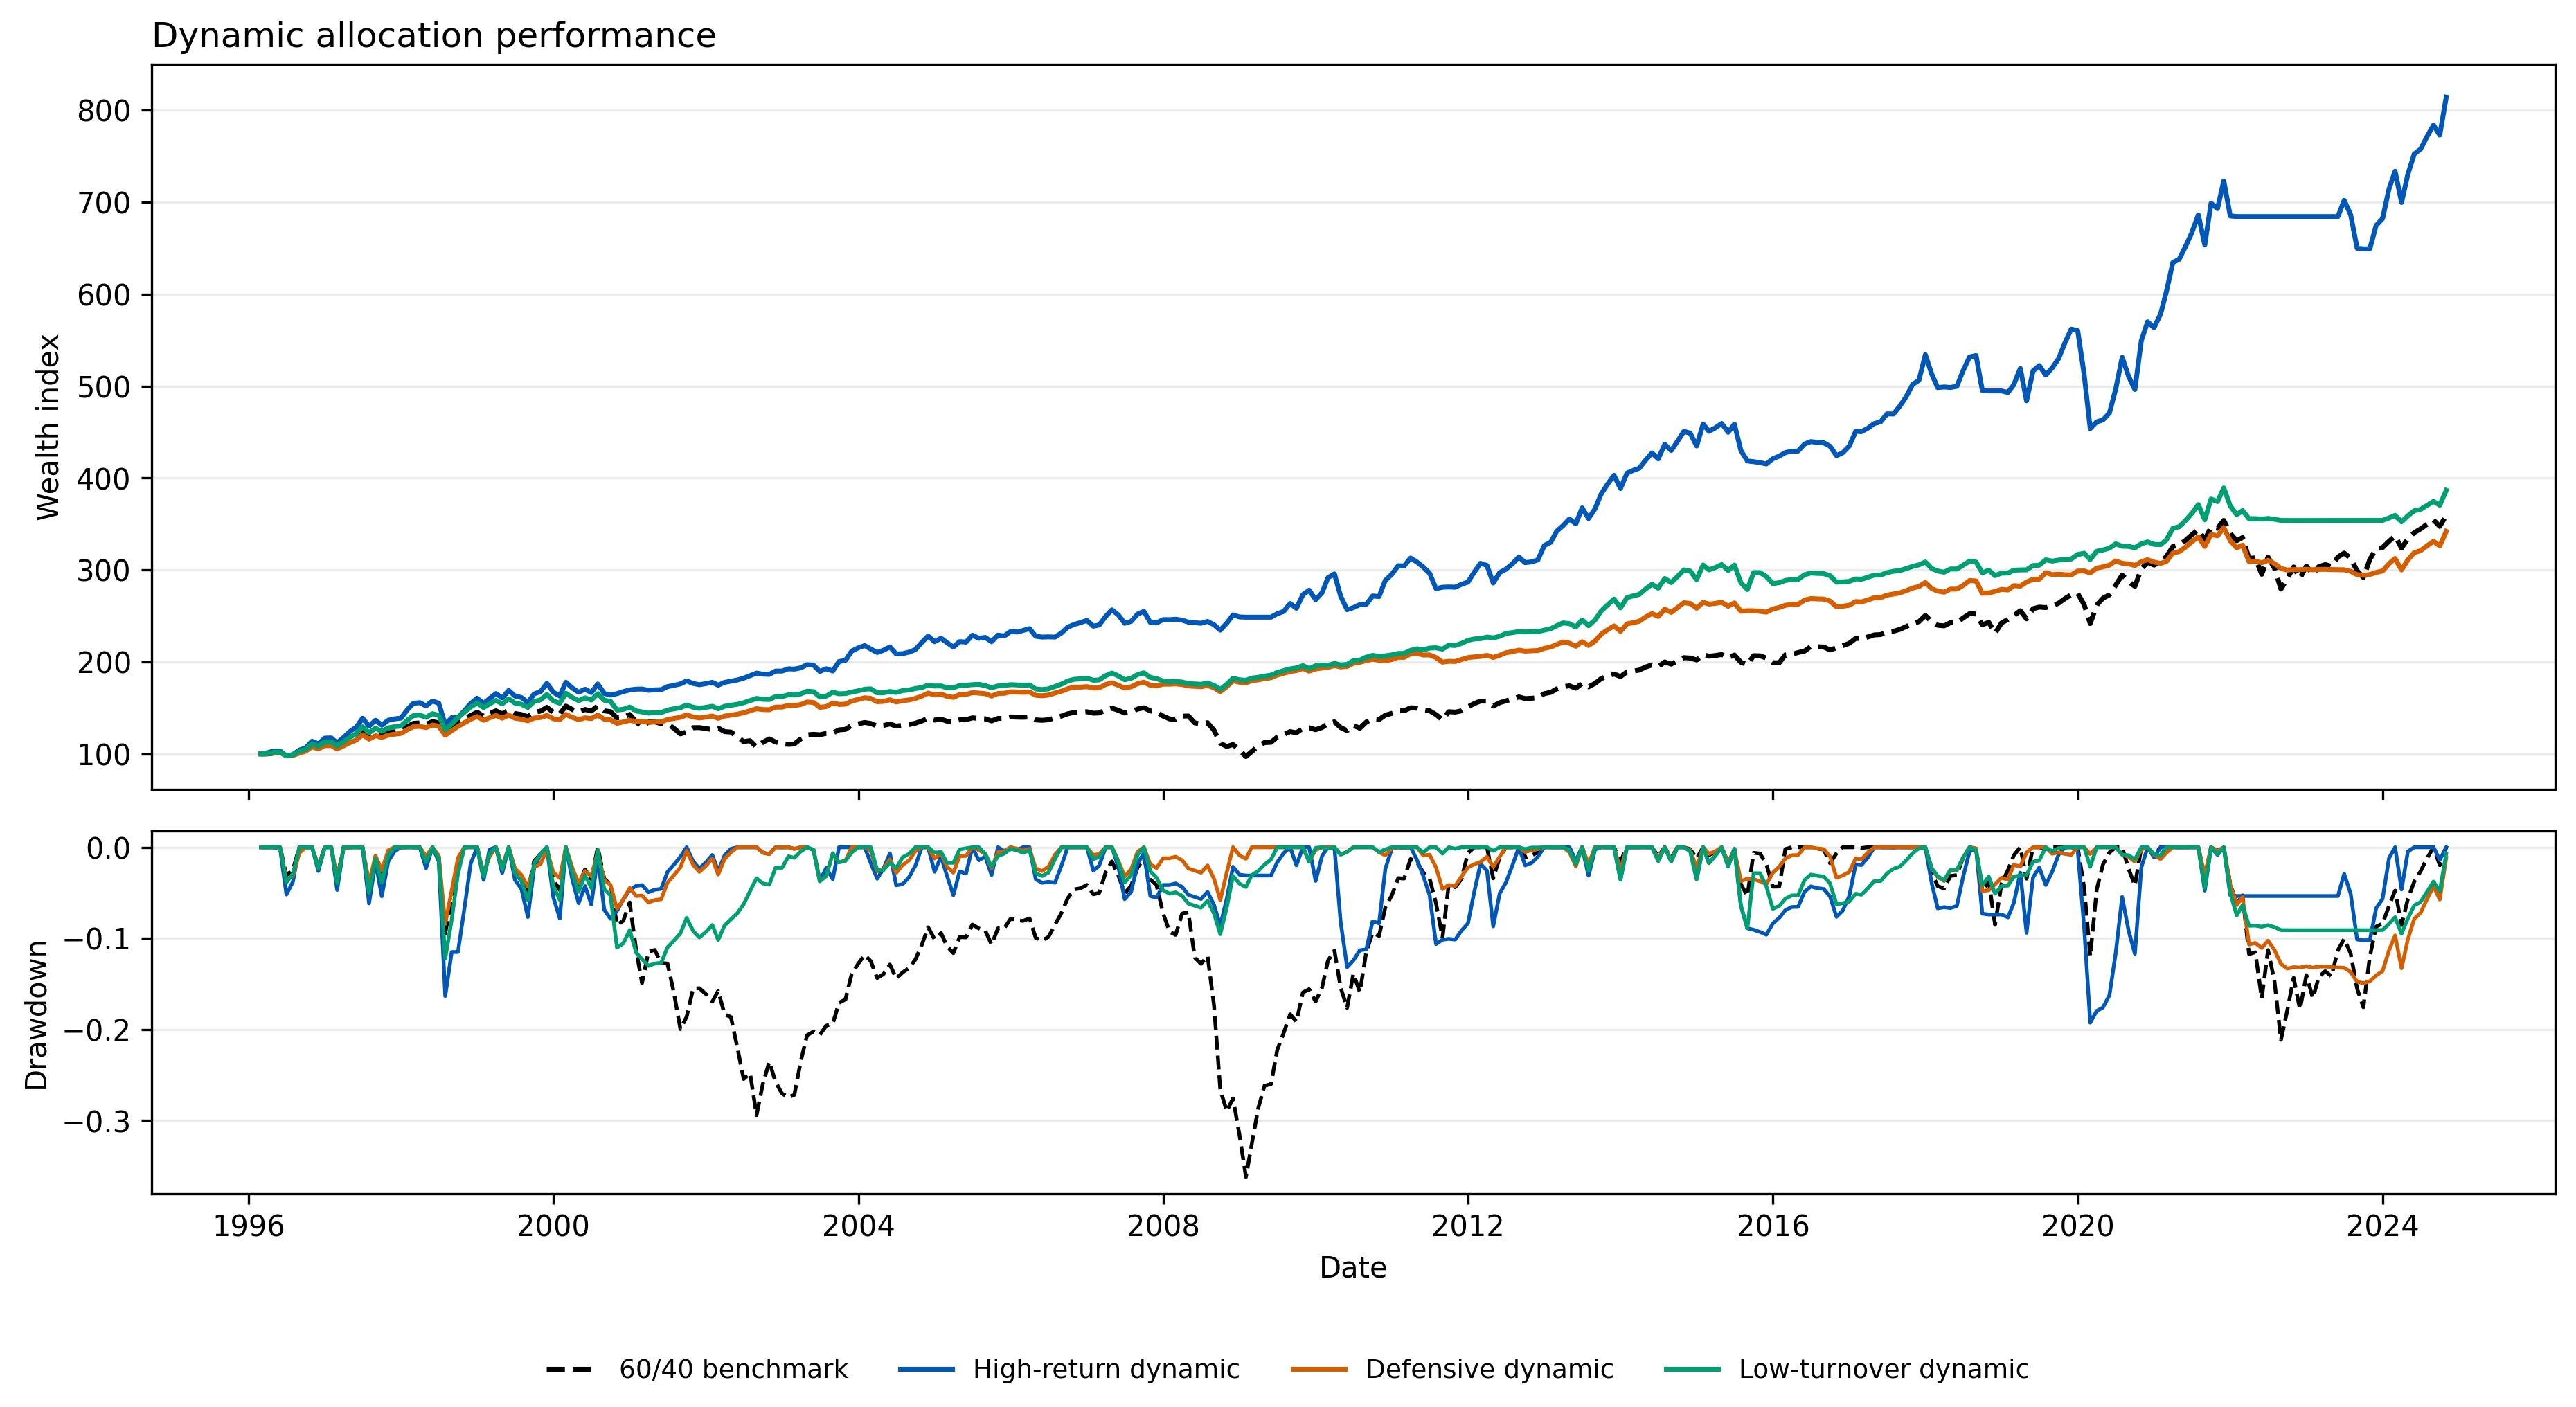
\includegraphics[width=\linewidth]{allocation_wealth_drawdown_focused.jpg}\\[2pt]
{\footnotesize\centering (a) \Bindep{}\par}
\end{minipage}\hfill
\begin{minipage}{0.5\textwidth}

\includegraphics[width=\linewidth]{COUPLED__alloc_wealth_drawdown.pdf}\\[2pt]
{\footnotesize\centering (b) \Acoup{}\par}
\end{minipage}
\caption{Dynamic allocation performance. The panels report wealth indexes and drawdowns for
the selected dynamic strategies and the 60/40 benchmark under the \Bindep{} and \Acoup{}
approaches.}
\label{fig:alloc-wealth}
\end{figure}

\subsection{Allocation mechanics}

The allocation mechanics show how the selected strategies use the probability forecasts.
Defensive strategies reduce risky exposure when adverse regimes receive higher probability.
This lowers volatility and drawdowns, with lower terminal wealth in strong equity markets.
High-return strategies keep larger risky positions for more of the sample and compound
faster in favourable periods. Low-turnover or balanced strategies make smaller reallocations
and sit between these two cases.

Figure~\ref{fig:alloc-mech} reports portfolio weights and turnover. In the \Bindep{} results,
the selected strategies differ in how they allocate across equity, bonds, and cash as the
equity and bond favourable-state probabilities change. In the \Acoup{} results, the weights
respond to the probabilities assigned to calm, normal, and stressed regimes. Across both
approaches, the main allocation channel is lower risky exposure during adverse regime
forecasts and greater use of bonds or cash when the predicted stock--bond environment
weakens.

\begin{figure}[H]
\centering
\begin{minipage}{0.48\textwidth}
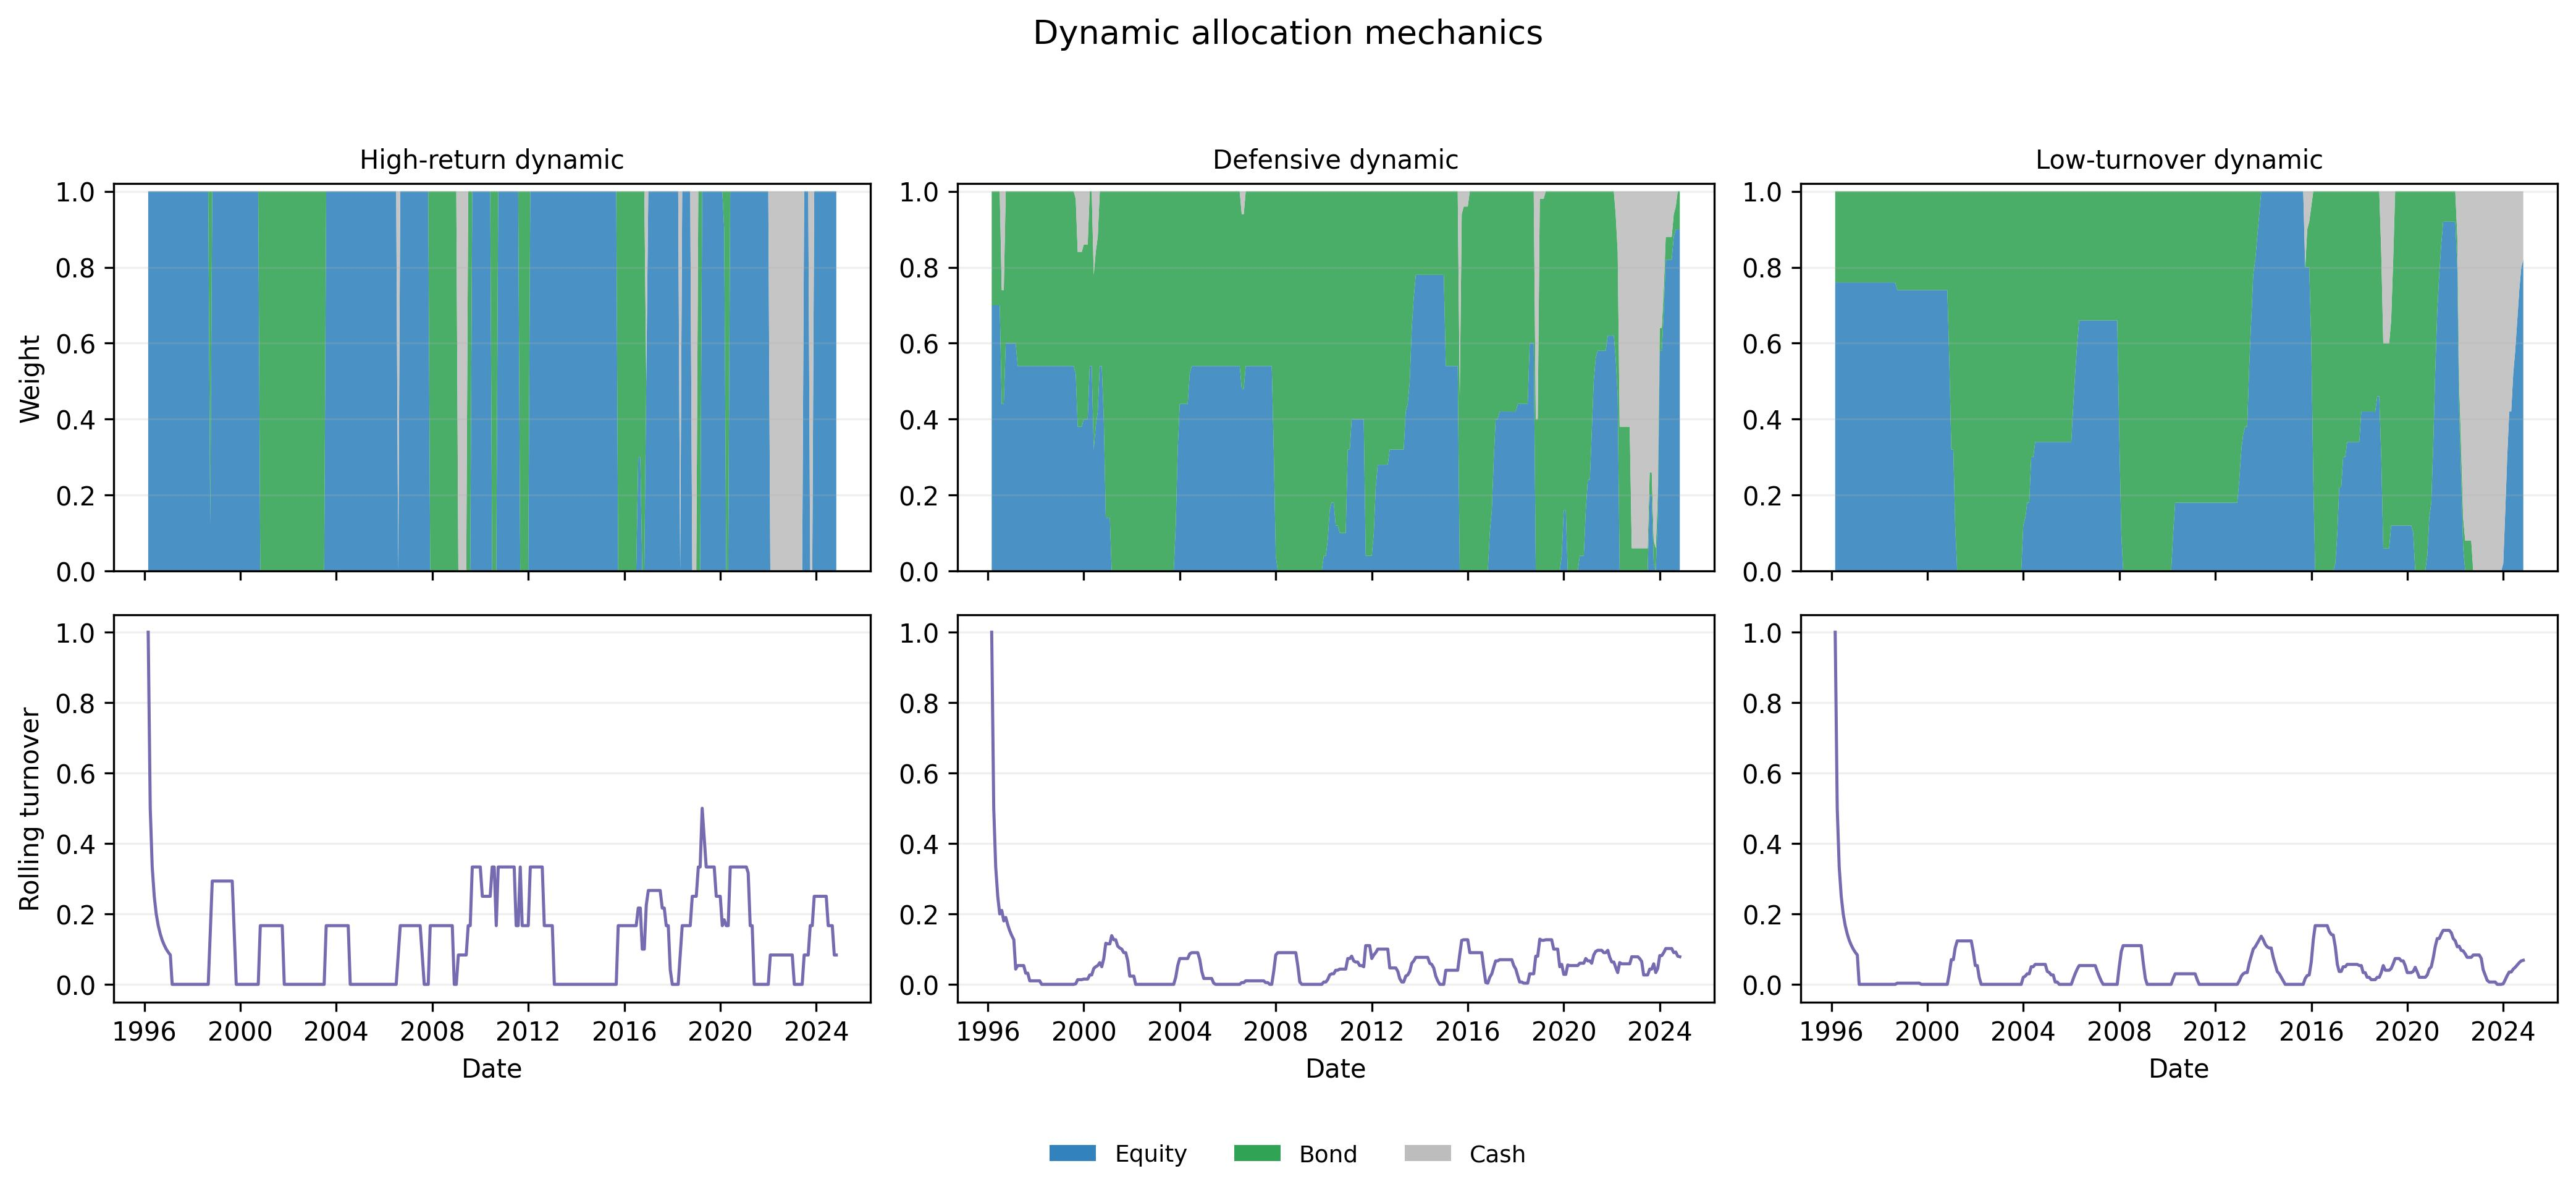
\includegraphics[width=\linewidth]{allocation_mechanics_focused.jpg}\\[2pt]
{\footnotesize\centering (a) \Bindep{}\par}
\end{minipage}\hfill
\begin{minipage}{0.5\textwidth}

\includegraphics[width=\linewidth]{COUPLED__alloc_mechanics.pdf}\\[2pt]
{\footnotesize\centering (b) \Acoup{}\par}
\end{minipage}
\caption{Dynamic allocation mechanics. The panels report portfolio weights and turnover for
the selected dynamic strategies under the \Bindep{} and \Acoup{} approaches.}
\label{fig:alloc-mech}
\end{figure}

\subsection{Sensitivity}

The sensitivity checks vary the main allocation parameters around the selected strategies.
In the \Bindep{} results, higher risk aversion lowers equity exposure and reduces drawdowns
in the defensive and low-turnover specifications. Probability smoothing reduces trading by
slowing changes in the forecast probabilities. Large turnover penalties reduce trading and
increase cash weights, with lower Sharpe ratios once the penalty becomes too large
(Table~\ref{tab:allocation-cost-turnover-sensitivity}).

The \Acoup{} sensitivity checks show the same trade-off between response strength and
trading cost. Raising risk aversion from \(\gamma=0.25\) to \(\gamma=5\) improves the
random-forest mean--variance Sharpe ratio from \(0.37\) to \(0.60\) and reduces annual turnover
from \(114\%\) to \(58\%\). The logistic Sharpe ratio is flatter over the same sweep, near \(0.60\).
For the turnover penalty, net Sharpe is highest around a small positive penalty and then
declines as the penalty becomes large. The probability-mixture mean--variance allocator's Sharpe ratio declines as
one-way transaction costs increase, from \(0.62\) at 5 bps to \(0.57\) at 25 bps
(Table~\ref{tab:c-cost}). Full parameter sweeps and cost tables are reported in
Appendices~\ref{app:alloc-independent} and \ref{app:alloc-coupled}. The independent-side
selection protocol is summarized in Appendix~\ref{app:independent-model-selection-protocol},
which separates fixed design choices, validation or grid-selected choices, and diagnostic
checks.

\section{Discussion and conclusion}
\label{sec:conclusion}

This paper studies monthly stock--bond allocation with regime labels that are estimated from realised asset-class returns and forecast from lagged macro-financial predictors. The empirical design has three stages. The teacher stage estimates persistent return environments for the equity and bond legs. The student stage forecasts the next-month teacher labels. The allocation stage converts the forecast probabilities into regime-conditional equity, bond, and cash weights with transaction costs and turnover control.

The comparison is between two regime representations. The \Bindep{} representation keeps separate binary favourable-state labels for equities and bonds. The \Acoup{} representation imposes a three-state joint stock--bond structure with calm, normal, and stressed regimes. The two representations answer related allocation questions. The independent labels give separate asset-level signals for equity and bond exposure. The coupled labels give a direct description of the joint diversification environment.

The teacher diagnostics show that both representations produce persistent and economically separated regimes. In the \Bindep{} labels, favourable equity and bond states have positive Sharpe ratios and unfavourable states have negative Sharpe ratios. In the \Acoup{} labels, calm has the strongest equity performance, normal describes equity weakness with bond support, and stressed describes joint adverse stock--bond conditions. The crisis-window evidence gives the main economic interpretation. Bonds support the portfolio in disinflationary equity drawdowns such as the dot-com bust and the global financial crisis. Bond protection weakens in inflation-driven episodes such as 1994 and 2022.

The student results show that the estimated regimes contain predictable structure in lagged macro-financial variables. For the independent labels, logistic regression gives the strongest headline AUC for both equity and bond favourable-state prediction. The feature-importance results differ by target: equity-regime forecasts depend strongly on equity cross-section and industry or style variables, while bond-regime forecasts use a broader mix of equity, Treasury, and credit information. This difference supports the asset-level design of the independent labels.

The allocation results provide the economic test of the forecasts. The dynamic strategies improve the 60/40 benchmark along different margins. Defensive specifications reduce maximum drawdowns and raise Sharpe ratios. Low-turnover or balanced specifications reduce trading intensity. High-return specifications increase terminal wealth while accepting larger drawdowns. These results show that the value of a regime forecast depends on the portfolio rule that converts probabilities into weights, including risk aversion, turnover penalties, transaction costs, smoothing, and moment shrinkage.

The evidence supports a state-dependent view of the stock--bond relation. A balanced portfolio benefits from bond exposure when weak equity returns coincide with positive bond performance. The same bond exposure can add risk when inflation shocks make equities and bonds decline together. The independent and coupled specifications give two complementary ways to represent this distinction: one through separate asset-level favourable-state probabilities, and one through a joint stock--bond regime label. In both cases, the forecast probabilities improve portfolio decisions when they are mapped into allocation rules that control turnover and trading costs.

\appendix
\renewcommand{\thefigure}{\thesection.\arabic{figure}}
\renewcommand{\thetable}{\thesection.\arabic{table}}

\input{appendix_body}

\end{document}
